\section{Station Metadata Dataset (GBFS)}

Our fourth source of data is the Lyft General Bikeshare Feed Specification (GBFS) feed\footnote{\url{https://gbfs.lyft.com/gbfs/2.3/bkn/en/gbfs.json}}, which provides current station information and live availability. Two endpoints are merged: \texttt{station\_information} (static metadata) and \texttt{station\_status} (real-time availability).

\subsection{Dataset Structure}

The station metadata dataset combines static station properties with live operational information. The static endpoint describes location and capacity, while the live endpoint reports availability and station status.

\subsubsection{Original Structure}

The merged dataset contains:

\begin{itemize}
    \item \textbf{From \texttt{station\_information} (static):}
    \begin{itemize}
        \item \textbf{Station ID}: numeric GBFS identifier.
        \item \textbf{Short Name}: public station identifier used for joins with Citi Bike trip data.
        \item \textbf{Name}: station name.
        \item \textbf{Latitude} and \textbf{Longitude}: station coordinates.
        \item \textbf{Capacity}: number of available docks.
    \end{itemize}

    \item \textbf{From \texttt{station\_status} (live):}
    \begin{itemize}
        \item \textbf{Bikes available}: currently rentable bikes.
        \item \textbf{Docks available}: currently available docks.
        \item \textbf{Operational flags}: \texttt{is\_installed}, \texttt{is\_renting}, and \texttt{is\_returning}.
    \end{itemize}
\end{itemize}

\subsubsection{Extracted Features}

An \texttt{active} indicator is derived from the three operational flags and is used to filter unavailable stations from live views.

\subsection{Analysis and Insights}
\begin{comment}
    Follows notebook 4.1 "Capacity and Live Availability" and 4.2 "Station Map".
    Per the exam requirements (Deliverable 2 - EDA criterion), the exploration below
    expands on three complementary perspectives: provisioning (capacity), current
    state (live bikes/docks), and spatial distribution (map). Each perspective
    connects directly to visualization design decisions for the final dashboard.
\end{comment}

The analysis focuses on station capacity, live availability, and spatial distribution.

Capacity distributions show how the network is provisioned, distinguishing small stations from larger hubs. Live availability of bikes and docks highlights possible imbalances, such as empty or saturated stations. The corresponding distributions are shown in Figure~\ref{fig:station_capacity}.

The station map provides a spatial overview of coverage and density, helping identify clusters, gaps, and possible coordinate issues. Capacity and availability values can also be used as visual encodings to improve the final dashboard, as shown in Figure~\ref{fig:station_map}.

\begin{figure}[ptb]
    \centering
    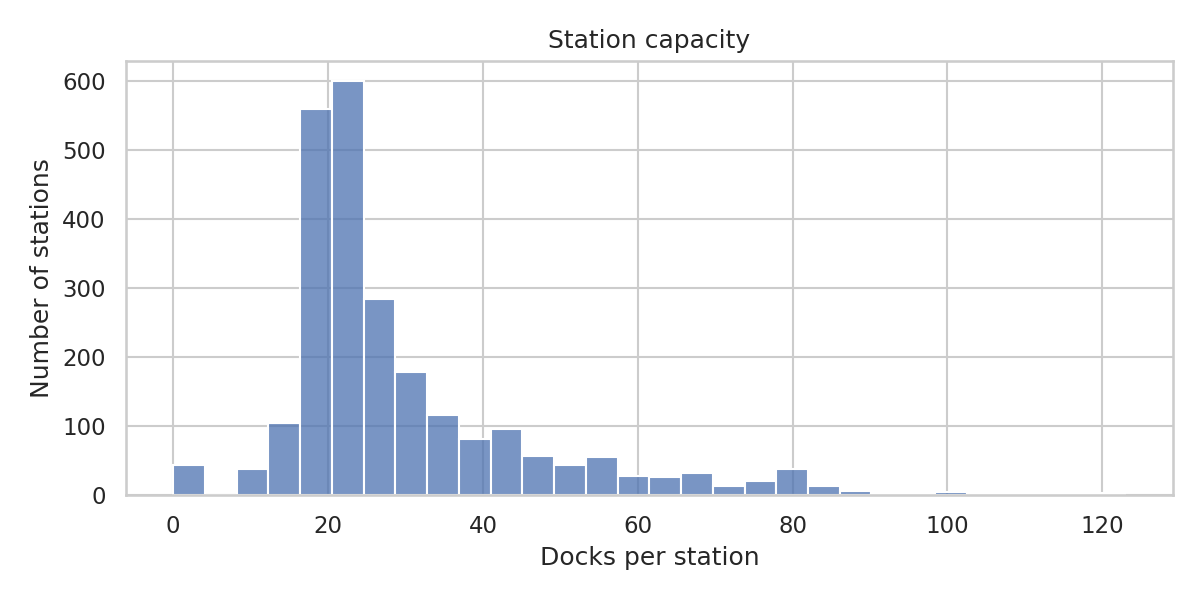
\includegraphics[width=\textwidth]{../media/station_capacity.png}
    \caption{Distribution of station capacity (number of docks) and live availability (bikes and docks available).}
    \label{fig:station_capacity}
\end{figure}

\begin{figure}[ptb]
    \centering
    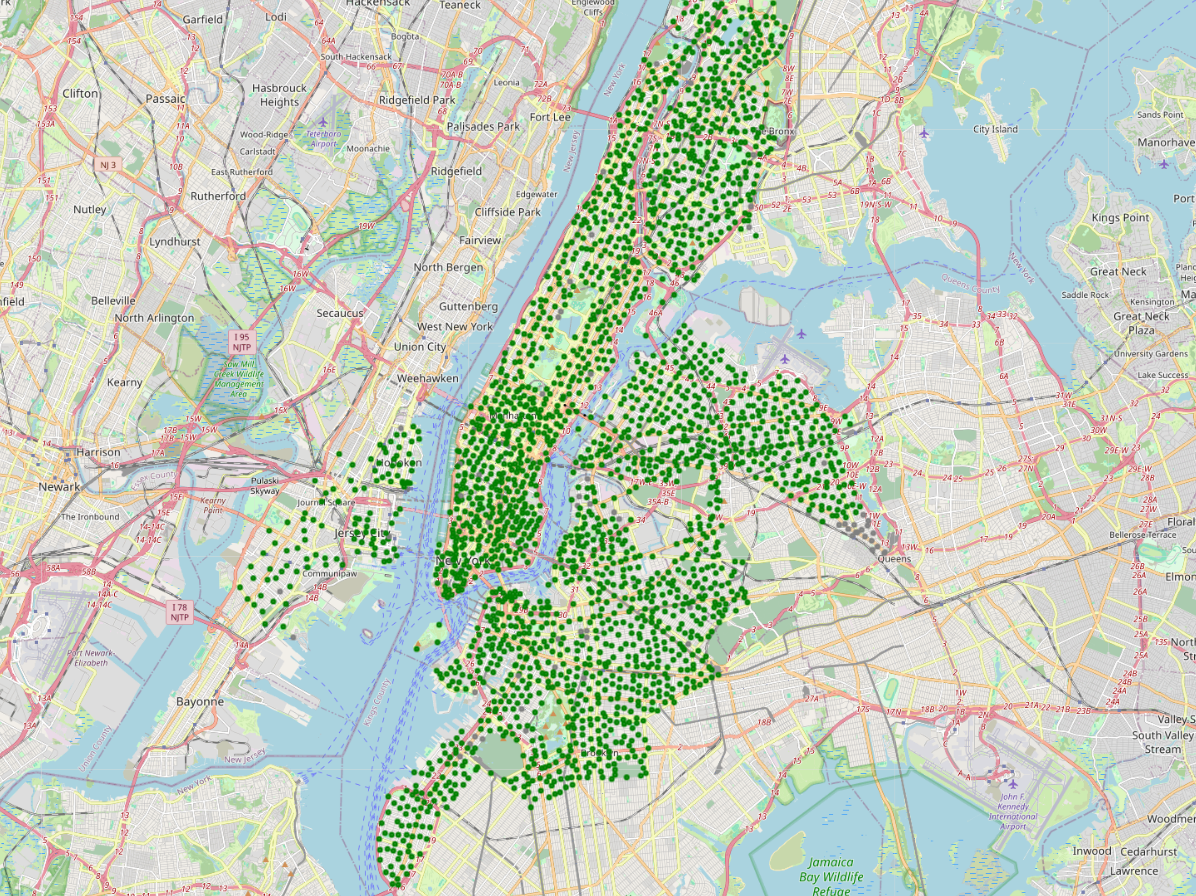
\includegraphics[width=.8\textwidth]{../media/station_map.png}
    \caption{Map of stations in New York City, colored by their active state.}
    \label{fig:station_map}
\end{figure}

\subsection{Data Quality}
\begin{comment}
    Follows notebook 4.3 "Data Quality". Per the exam requirements (Deliverable 2 -
    data quality criterion), discuss:
      - Count of inactive stations (not installed/renting/returning) that need to be
        filtered out of live views.
      - Stations missing capacity or coordinates.
      - Cross-dataset consistency issue: the numeric station_id (GBFS) differs from
        the public short_name used in the Citi Bike trip files, so joins between
        live station data and historical trips must go through short_name rather
        than station_id. This connects back to the "Missing Values and
        Inconsistencies" discussion in the City Bike chapter.
\end{comment}

The main quality issues concern station status, missing attributes, and identifier consistency.

Some stations are present in the feed but not fully operational because one or more status flags are false. These stations are excluded from live visualizations using the derived \texttt{active} feature.

A small number of records may have missing capacity or coordinates. Stations without coordinates cannot be displayed on maps, while missing capacity only affects analyses based on station size.

Cross-dataset joins require attention because GBFS provides both a numeric \texttt{station\_id} and a public \texttt{short\_name}. Historical trip data use \texttt{short\_name}, therefore all joins are performed using this field after validating its consistency.

Additional issues, such as temporary feed outages or duplicate identifiers caused by station changes, are handled through preprocessing checks to maintain reliable visualizations.